\section{Bloque 4}\label{bloque-4}

En este bloque del trabajo vamos a realizar un ataque a un sistema de
control de acceso real que use RFID. Intentaremos averiguar cómo
funciona, qué tecnología usa, que protocolos se usan, etc. buscando
información en Internet y mediante la ingeniería inversa. En este bloque
se detallará paso a paso todo lo que hemos hecho.

\subsection{Qué sistema real podemos
atacar}\label{quuxe9-sistema-real-podemos-atacar}

La primera cuestión que nos planteamos es dónde podemos encontrar un
sistema que use RFID y que tengamos acceso a él para ejecutar el ataque.
Tras pensar en varias posibilidades pensamos que la más interesante
podría ser el Bonobús de Tussam.

El Bonobús es una tarjeta que usa la tecnología RFID para comunicarse
con las canceladoras que podemos encontrar en todos los autobuses.
Funciona como una tarjeta monedero ya que contiene un saldo que se va
decrementando al pasar por la canceladora y se puede recargar en los
puntos oficiales. Nuestro objetivo será buscar posibles debilidades en
el sistema para poder pasar por el sistema de control de acceso sin
necesidad de recargar el Bonobús.

\subsection{Funcionamiento del Bonobús de Tussam y MIFARE
Classic}\label{funcionamiento-del-bonobuxfas-de-tussam-y-mifare-classic}

Lo primero de todo será saber a qué nos enfrentamos. Qué tecnología usa
el Bonobús de Tussam. Basta una rápida búsqueda en Internet para ver que
el Bonobús ha sido diseñado por Indra y los TAGs usan la tecnología
MIFARE. En concreto los TAGs son MIFARE Classic 1K. En Internet hay
abundante información de estos chips y cómo funciona su sistema de
seguridad, a continuación intentaremos explicar brevemente su
funcionamiento.

\subsubsection{MIFARE Classic 1K}\label{mifare-classic-1k}

La tecnología Mifare Classic es una de las más utilizadas en entornos de
producción (sistemas de ticketing, control de acceso físico, monedero
electrónico, etc.). El proceso de análisis de la seguridad de este tipo
de tarjetas ha sido realizado por la Universidad Nijmegen Holandesa en
2008, consiguiendo romper el cifrado propietario de Philips CRYPTO1
sobre el cual se basa Mifare. El problema reside en la predictibilidad
del algoritmo de generación de números aleatorios, como ocurre en otras
tecnologías.

Antes de entrar en los detalles técnicos de las debilidades de
seguridad, pasaremos a describir su funcionamiento y estructura. En una
arquitectura básica Mifare encontramos un lector y un TAG o tarjeta,
ejerciendo una comunicación dentro del radio de acción inalámbrico (unos
5 cm). Mifare Classic está basado en el estándar ISO 14443 e incorpora
un protocolo anticolisiones, es decir, permite trabajar con varias
tarjetas que estén dentro del radio de acción del lector al mismo
tiempo. La principal diferencia de la implementación de Philips frente
al estándar ISO 14443 es que la comunicación se produce de forma cifrada
tras un proceso de autenticación mutuo lector-tarjeta. Cada 8 bits de
transmisión, uno se utiliza para calcular la paridad, pero este es
cifrado también, dejando la comprobación de integridad a la capa de
aplicación.

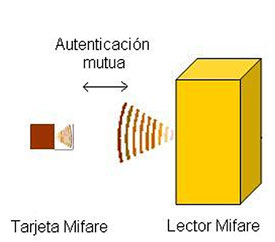
\includegraphics{memoria/images/fig4-1.jpg}

Por lo que a su estructura lógica se refiere, la tarjeta está
representada como un mapa de memoria con bloques de datos de 16 bytes.
Estos bloques de datos se agrupan en sectores. Aquí hay que diferenciar
las tarjetas de 1k de las de 4k.

Las de 1K tienen 16 sectores con 4 bloques de datos cada uno. El último
bloque de datos de cada sector se denomina trailer y es donde se
guardarán las claves privadas de acceso y los permisos para acceder a
ese sector, lo veremos más en detalle a continuación.

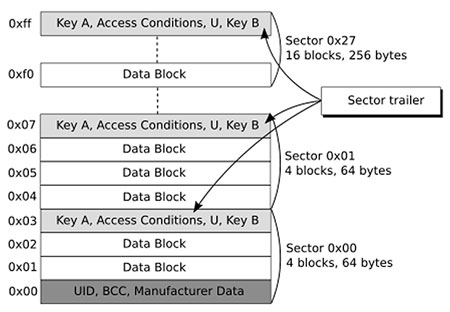
\includegraphics{memoria/images/fig4-3.jpg}

Por último cabe destacar que existe un bloque especial que esta
localizado en el bloque de datos 0 del sector 0, que alberga la
siguiente información en modo solo lectura:

\begin{itemize}
\itemsep1pt\parskip0pt\parsep0pt
\item
  UID: Identificador único de la tarjeta.
\item
  BCC: bit count check, calculado por la sucesivas XORs de los bytes del
  UID.
\item
  11 bytes de datos que identifican al fabricante del tag.
\end{itemize}

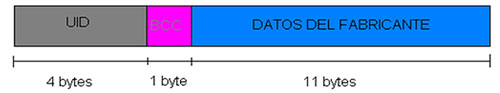
\includegraphics{memoria/images/fig4-2.jpg}

Para que el lector pueda leer y escribir el contenido de un sector, es
decir, cualquiera de los 4 bloques de datos que tiene, necesita en
primera instancia autenticarse contra él. Este proceso se realiza si y
solo si la clave utilizada por el lector coincide con la que el sector
trailer alberga. Mifare permite la utilización de dos claves por sector,
la Key A (6 bytes) y la Key B (6 bytes), donde las condiciones o
permisos de acceso al sector los marca la máscara Access Conditions (3
bytes). El byte restante U no tiene propósito específico. Este sistema
permite con una única tarjeta desplegar varios sistemas que puedan
interactuar con ella de forma independiente y sin conocer los datos de
otros sectores. De esta manera, por ejemplo, una empresa de telefonía
podría desplegar su sistema de monedero electrónico sin interferir en
otro sistema de control de acceso físico implementado por un segundo,
entregando al usuario un único Token de actuación.

Comencemos profundizando un poco más en como Mifare realiza el proceso
de autenticación. En primera instancia el lector le comunica a la
tarjeta que quiere realizar una operación sobre un sector de datos
determinado N. El TAG o tarjeta en ese momento remite un número
aleatorio Nc (Nonce del cliente) de 32 bits a modo de reto, para que sea
cifrado con la clave privada compartida previamente. Como respuesta, el
lector remite el reto cifrado y un número aleatorio Nr (Nonce del
lector) para que el TAG lo cifre con la clave privada, generando una
trama de 64 bits. En última instancia la tarjeta le envía al lector su
reto cifrado. En este momento ambos tienen la certeza de que los
dispositivos son legítimos. Destacar que los dos últimos intercambios se
realizan ya de forma cifrada, permaneciendo en claro tan solo el envío
de la petición de lectura y Nc.

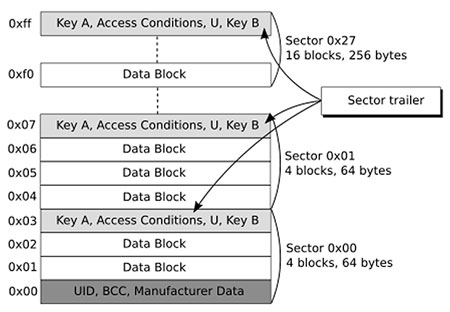
\includegraphics{memoria/images/fig4-3.jpg} Handshake.

\subsubsection{Ataques a Mifare Classic}\label{ataques-a-mifare-classic}

Una vez conocido el funcionamiento de nuestro TAG en cuestión es obvio
que lo que necesitamos es averiguar cuáles son las claves A y/o B de los
diferentes sectores de nuestro TAG. Para ello existe diferentes ataques
posibles que explicamos a continuación.

\paragraph{Sniff}\label{sniff}

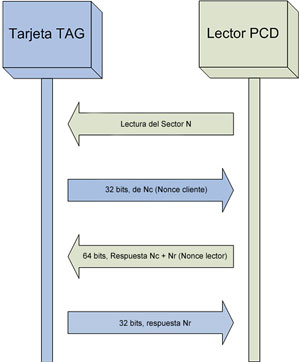
\includegraphics{memoria/images/fig4-4.jpg}

¿Cómo podemos capturar una comunicación real entre un tag y un lector?
Para ello necesitamos usar un dispositivo que nos permita realizar
sniffing a la tecnología ISO14443 tipo A sobre la que se basa Mifare.

Ya que tenemos el dispositivo que nos permitirá capturar el handshake
inicial entre la tarjeta y el lector, ahora tan solo nos falta un lector
MIFARE y un TAG. Para el lector debemos ir con el dispositivo a las
canceladoras en los autobuses o a los puntos de recarga. Para la tarjeta
se usaría el Bonobús tal cual.

Colocando el sniffer entre la tarjeta y el lector podríamos proceder a
realizar una lectura del sector 4, obteniendo la siguiente traza de
bytes.

\% Imagen de una captura

Es conveniente comentar ciertos aspectos de la captura:

\begin{itemize}
\itemsep1pt\parskip0pt\parsep0pt
\item
  En primer lugar ETU corresponde con Elementary Time Units, y define el
  tiempo entre mensajes, donde 1 ETU corresponde con un cuarto del
  período de bit, que es igual a 1,18 microsegundos.
\item
  SEQ en este caso correspondería con el número de mensaje.
\item
  La trama ``2a 69 8d 43 8d'' identifica la tarjeta Mifare dentro del
  rango del lector, este identificador es pregrabado en el sector 0 del
  tag y no es modificable.
\item
  El byte ``60'' de la secuencia ``07'' indicaría a la tarjeta que se
  pretende trabajar y por tanto autenticar, en un sector determinado, en
  este caso el sector 01 donde esta albergado el bloque de datos 04
  (siguiente byte al ``60'') y utilizando para ello la clave A. Si nos
  encontráramos con un valor ``61'' se trataría de un intento de
  autenticación utilizando la clave B del sector.
\item
  El resto de tramas que implican el proceso de autenticación ya han
  sido comentadas anteriormente (Nc, Nr, Rc, Rr).
\end{itemize}

\begin{verbatim}{Explicación de la debilidad de CRYPTO1}\end{verbatim}

Con la información anterior capturada procederemos a inferir la clave
privada del sector mediante la aplicación CRAPTO1 de desarrollo anónimo
(lógico dado los problemas que tuvo la universidad de Radboud con
Philips por su investigación).

Configuramos crapto1 con los parámetros anteriores:

\begin{itemize}
\item uid
\item tag\_challenge
\item nr\_enc
\item reader\_response
\item tag\_response
\end{itemize}

Tras ejecutar el programa obtenemos la clave.

Con esta clave privada ya podemos pasar a leer/modificar el contenido de
los 4 bloques de datos que componen el sector 01, podríamos por ejemplo,
cambiar esta clave privada escribiendo en el bloque de datos trailer o
incrementar el valor de nuestro monedero electrónico. Cuidado al
realizar esta primera operación, ya que podríamos modificar el tipo de
acceso (3 bytes de Acces Conditions) y dejar el sector inservible.

El problema pricipal de este ataque es que hay que desplazarse hasta la
canceladora del autobús con todos el dispositivo y un ordenador para
poder usarlo. Aunque podría hacerse de forma disimulada, en nuestro caso
hemos usado otro ataque por ser mucho más viable y no requerir la
presencia de la canceladora.
